\clearpage
\subsection{String} % (fold)
\label{sub:string}

Textual data is stored as an array of characters. 

\begin{figure}[h]
   \centering
   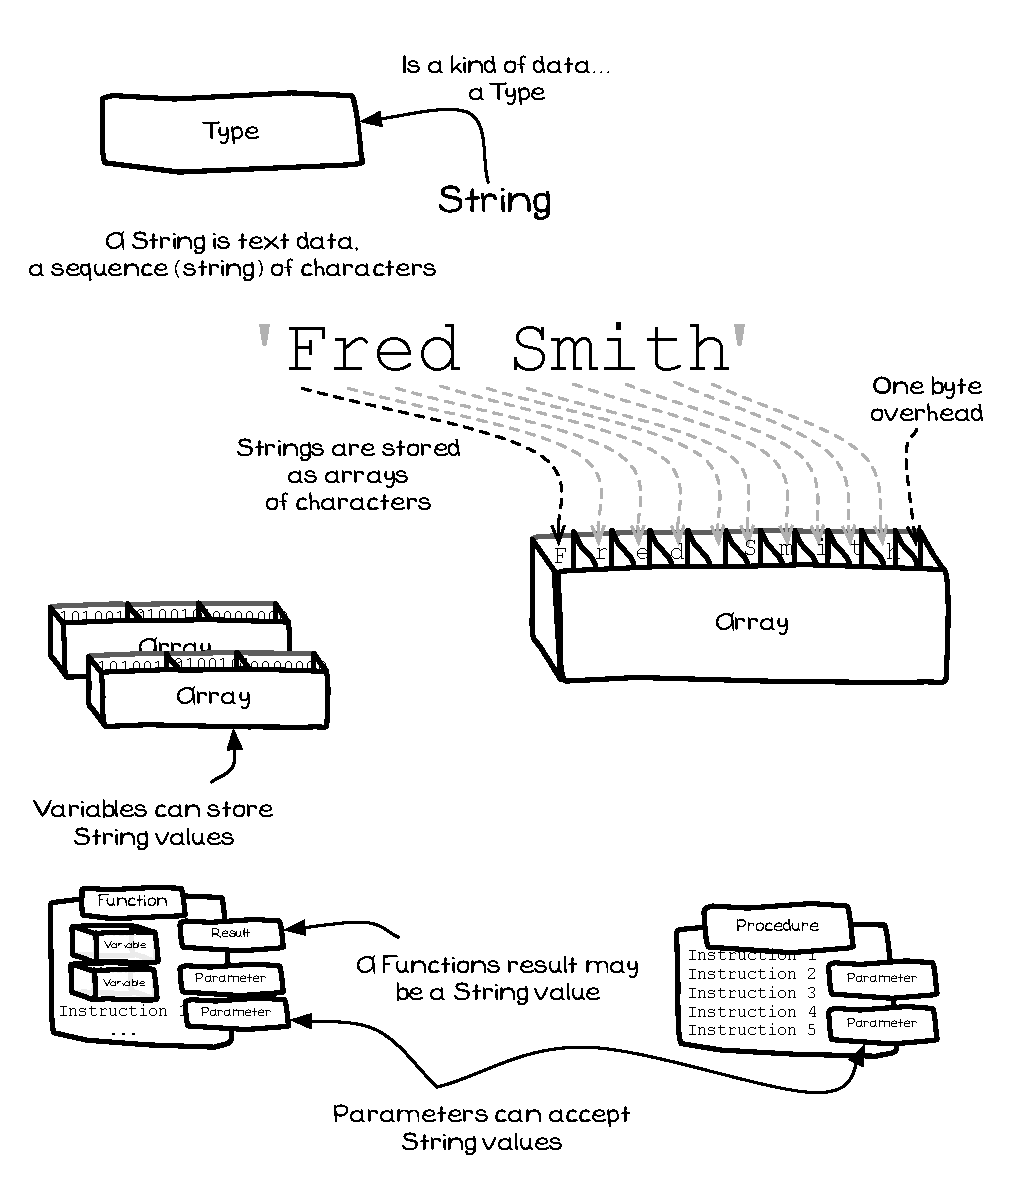
\includegraphics[width=0.8\textwidth]{./topics/arrays/diagrams/String} 
   \caption{Strings are textual data, stores as an array of characters}
   \label{fig:strings}
\end{figure}

\mynote{
\begin{itemize}
  \item Boolean is an existing \textbf{artefact}, it is a \nameref{sub:type} that has been defined to represent text values.
  \item A string is an array of characters.
  \item Both C and Pascal have additional overhead in the string data. In C the overhead is used to store a single terminating character that indicates the end of the string, in Pascal this stores the number of characters.
\end{itemize}
}

\csection{C does not have a native String type, instead you use an array of characters. As a result, C has very limited support for string data. For details see \nameref{sub:c_string}.}

% subsection string_type (end)